\section{Data Collection}

\subsection{Pre-processing}

\begin{figure}[H]
		  \centering	
          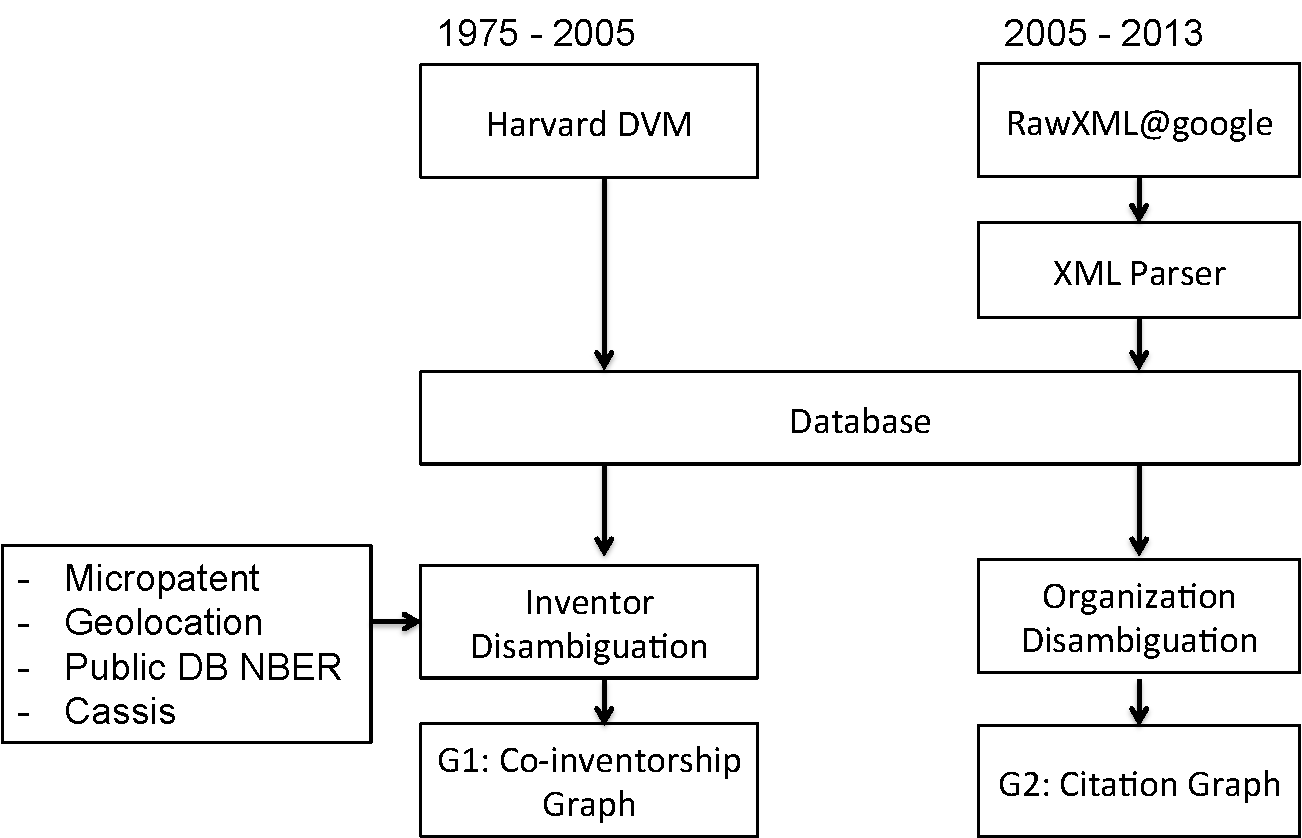
\includegraphics[scale=0.6]{../figures/process.pdf}
          \caption{This is the second figure}
\end{figure}

\subsection{Author Disambiguation}

\subsection{Organisation Disambiguation}

\begin{table*}[h] 
  \centering
  \begin{tabular}{@{}c@{}} 

  \begin{minipage}{0.25\linewidth}

\begin{lstlisting}[]
<node id="n196819">
  <data key="Loc">BOZEMAN-MT-US</data>
  <data key="Name">BERG, LLOYD</data>
  <data key="id">04292142-1</data>
  <data key="Patents">247</data>
</node>
\end{lstlisting}

  \end{minipage}
  \hspace{0.05\linewidth}
  \begin{minipage}{0.3\linewidth}

\begin{lstlisting}[]
<node id="n471405">
  <data key="Loc">BOZEMAN-MT-US</data>
  <data key="Name">EDISON, THOMAS A</data>
  <data key="id">05147512-2</data>
  <data key="Patents">1</data>
</node>
\end{lstlisting}

  \end{minipage}
  \hspace{0.05\linewidth}
  \begin{minipage}{0.3\linewidth}

\begin{lstlisting}[]
<edge source="n196819" target="n471405">
  <data key="tId">05147512-2</data>
  <data key="hId">04292142-1</data>
  <data key="AppYear">1991</data>
  <data key="Weight">1</data>
</edge>



\end{lstlisting}

  \end{minipage}
  
  \end{tabular}

\label{listing}
\caption{\footnotesize Snippet from GraphXML. Shows the nodes for Lloyd Berg and Thomas Edison and the corrsponding edge between them.}
\end{table*}